% Source: 文章_bu1118.docx, Introduction only.
\section{Introduction}
\label{sec:introduction}

Vision-Language-Action (VLA) models have become a core paradigm for general-purpose embodied AI by mapping multimodal perceptions and language instructions into robot actions. However, practical VLA deployment faces severe challenges. While VLA inference must meet strict real-time constraints to avoid task failure, the physical limits of robots restrict deployment to edge platforms with constrained power, compute, and memory bandwidth, such as the LPDDR-equipped NVIDIA Orin and Thor. Taking the representative $\pi_{0.5}$ model~\cite{pi05} as an example, its inference latency on NVIDIA Thor reaches about $141\,\mathrm{ms}$ ($7\,\mathrm{Hz}$), limiting the robot's control frequency.

From a workload perspective, VLA models show heterogeneity in computation and memory access~\cite{vla_perf}. A typical VLA model cascades a Vision-Language Model (VLM) and an Action Expert (AE), with an execution time ratio of about 1:1 to 1:2 (\textbf{Fig.~\ref{fig:intro-overlap}(a)}). As embodied robot control dictates single-batch inference, the large difference in input token lengths between the two networks leads to distinct operational intensities (OI). Profiling on NVIDIA Thor shows that the AE is severely memory-bound, while the VLM lies near the boundary between the compute- and memory-bound regions (Section~\ref{sec:background-a}). Although recent works decouple sequential VLM--AE execution into asynchronous parallel execution to hide latency~\cite{vla_xpu,ravel}, single-GPU concurrency fails to exploit this algorithmic parallelism because streaming the AE saturates the off-chip memory bandwidth, achieving only a $1.03\times$ speedup via dual-stream execution on NVIDIA Thor (\textbf{Fig.~\ref{fig:intro-overlap}(b)}).

% Source: figures/sources/figures1107-20261118.pdf, page 1.
% PDF content retained; only blank page borders cropped.
\begin{figure}[!tb]
\centering
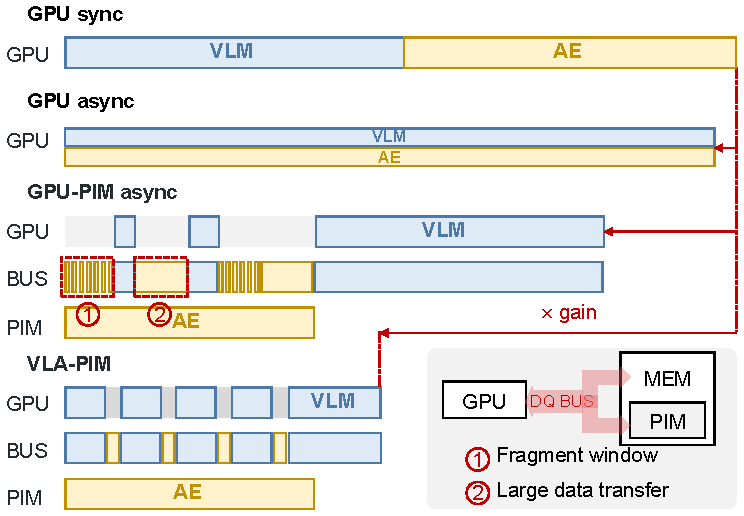
\includegraphics[width=\columnwidth,pagebox=cropbox]{figures/execution-overview.pdf}
\caption{VLA execution paradigms: serial GPU execution, GPU--PIM overlap limited by fragmented bus windows and data transfers, and VLA-PIM.}
\label{fig:intro-overlap}
\end{figure}


Achieving effective VLM--AE parallelism for such heterogeneous workloads requires heterogeneous hardware. DRAM Processing-in-Memory (PIM)~\cite{rowclone,ambit,fimdram,upmem_prism} can efficiently accelerate memory-bound workloads by computing near the memory arrays. Therefore, replacing the edge GPU's standard LPDDR with LPDDR-PIM offers an attractive heterogeneous solution: LPDDR-PIM can supply main-memory data to the GPU for VLM execution while concurrently computing the memory-bound AE in memory to hide latency.

However, because GPU memory accesses and PIM transfers share the same command/address (C/A) and data (DQ) buses of the LPDDR interface, efficient GPU--PIM concurrency is severely limited by shared-bus contention (\textbf{Fig.~\ref{fig:intro-overlap}(c)}). This contention stems from two main aspects. First, PIM's streaming input and execution leave highly fragmented bus idle windows. Overly short windows cannot accommodate complete GPU memory accesses, while fragmented windows force frequent PIM-to-GPU rank switching, incurring high turnaround overhead. Second, massive inter-rank PIM data movement heavily occupies the bus. Specifically, executing the AE on PIM involves matrix transposition, data rearrangement, broadcast, and partial-sum reduction, all of which require frequent inter-rank communication.

Prior GPU--PIM coordination techniques cannot resolve this contention under edge LPDDR constraints. Some designs (e.g., AHASD and LP-Spec~\cite{ahasd,lp_spec}) add cross-rank global schedulers and memory controllers (MCs) that rely on a \emph{logic die}, which is absent in commercial LPDDR and Samsung's LPDDR-PIM~\cite{samsung_lpddr5x_pim}. Other designs that invasively modify internal bank circuits on the DRAM die for concurrent access and computation (e.g., NeuPIMs~\cite{neupims}) incur prohibitive area overhead, over $10\times$ higher than logic-die implementations~\cite{sangam,devaux}.

In this work, we present VLA-PIM (\textbf{Fig.~\ref{fig:intro-overlap}(d)}), the first heterogeneous GPU-LPDDR5X-PIM system that accelerates edge VLA inference through architecture--dataflow co-design. Specifically, VLA-PIM employs rank-level partitioning to isolate memory resources between GPU accesses and PIM computation (Section~\ref{sec:architecture-a}). Furthermore, an input-preloading microarchitecture (Section~\ref{sec:architecture-b}) and a DQ-aware dataflow (Section~\ref{sec:dataflow-a}) mitigate shared-bus contention, effectively overlapping AE computation with VLM execution. Notably, VLA-PIM requires neither a \emph{logic die} nor invasive bank modifications while matching the compute and local-buffer budgets of Samsung's LPDDR-PIM, ensuring practical hardware feasibility. Our contributions are summarized as follows:

\begin{itemize}
\item We characterize the distinct OI of the VLM and AE, and introduce a heterogeneous execution paradigm that runs the VLM on the GPU and the AE on PIM in parallel.
\item We propose the VLA-PIM architecture, which employs rank-level resource partitioning to isolate GPU memory accesses for the VLM from in-memory PIM execution for the AE with minimal hardware overhead.
\item We design an input-preloading microarchitecture to eliminate fragmented bus windows, alongside a DQ-aware dataflow to minimize inter-rank traffic on the shared bus.
\end{itemize}

We build and open-source a Ramulator-based cycle-accurate simulator~\cite{ramulator2} to evaluate VLA-PIM, demonstrating a $1.82\times$ speedup and a $2.52\times$ energy reduction over a serial GPU baseline.
